\section{IP (Network Layer)}

\subsection{Router/Gateway}
Verbinden verschiedene Netze mit potentiell unterschiedlichen Technologien

Lösen 2 Aufgaben:
\begin{description}
	\item[Routing] Aufbau und Update von Routingtabellen
	\item[Forwarding] Weiterleiten der Pakete anhand Routingtabellen
\end{description}

\subsubsection{Routing-Tabelle}
löst: wie Kann ich welches Netz erreichen?

Bei hierarchischem Routing (Router wissen welche Netze an anderen Router sind
forwarden entsprechend) kommen oft auch aggregierte Routen vor.\\
Wenn so z.B. 130.0.0.0/25 und 130.0.128.0/25 beide via den selben Router
erreichbar sind wird diese Route aggregiert und als 130.0.0.0/24 zusammengefasst.

\begin{center}
	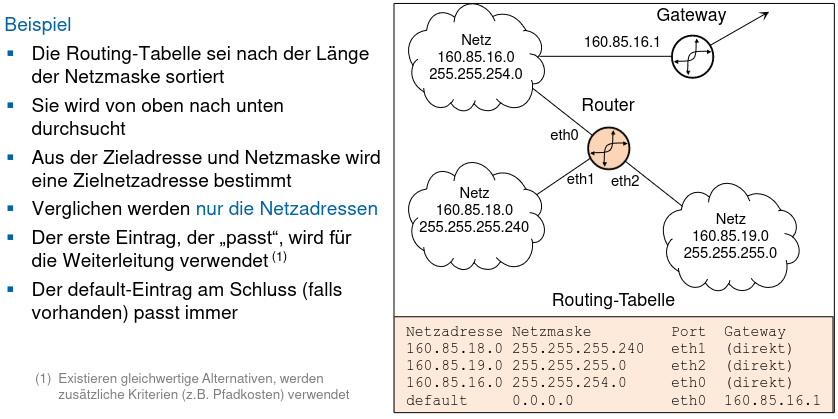
\includegraphics[width=0.9\linewidth]{routing-table}
\end{center}

\subsubsection{Classful Routing}

Ursprünglich wurden IP Adressen in 5 Routing Klassen eingetelt (Classful Routing).
Die ersten vier Adressbits erlauben eine Bestimmung der Klasse.
Wird nicht mehr gemacht weil oftmals Adressraum verschwendet wird.

\begin{center}
	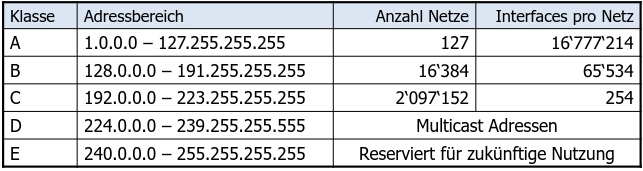
\includegraphics[width=0.9\linewidth, height=15mm]{classful-routing}
\end{center}

\subsubsection{Subnetting}
\begin{itemize}
	\item das Netz in kleinere Subnetze teilen
	\item funktioniert simplifiziert durch beliebiges erweitern der Netzadresse
	\item hintereinanderliegende Netze können zusammengefügt werden
	      \begin{center}
		      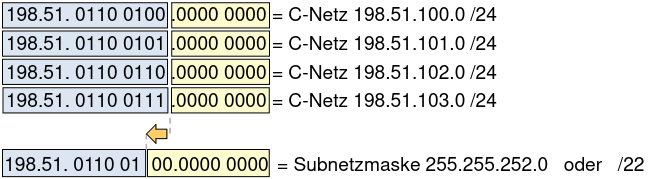
\includegraphics[width=0.8\linewidth, height=10mm]{subnetting-aggr}
	      \end{center}
	      % \begin{itemize}
	      %  \item 160.85.100.0/24
	      %  \item 160.85.101.0/24
	      %  \item 160.85.102.0/24
	      %  \item 160.85.103.0/24
	      %  \item zusammengefügt: 160.85.100/22
	      % \end{itemize}
\end{itemize}








\subsection{Adressierung / IPv4}

Adresse eines Host = Netz-Adresse + Interface-Adresse

\subsubsection{Subnetzmaske}

\begin{center}
	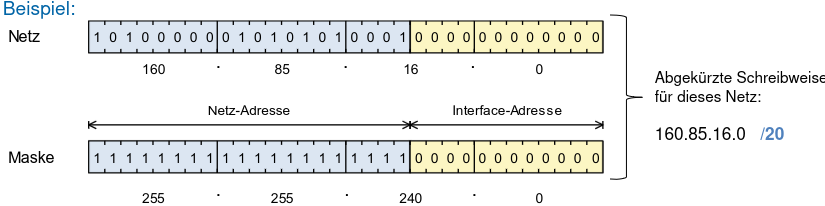
\includegraphics[width=0.9\linewidth]{subnetmask}
\end{center}

\subsubsection{Netzadresse}

\begin{itemize}
	\item reserviert, darf NICHT für interfaces verwendet werden
	\item tiefste Adresse im Subnet $\rightarrow$ alle interface bits 0
	\item berechnung durch $Interface Adresse \land Subnetzmaske$
\end{itemize}

\subsubsection{Broadcast-Adresse}

\begin{itemize}
	\item reserviert, darf NICHT für interfaces verwendet werden
	\item höchste Adresse im Subnet $\rightarrow$ alle interface bits 1
	\item berechnung durch $Interface Adresse \lor invertierte \, Subnetzmaske$
\end{itemize}

\subsubsection{Private Adressen}

Die $172.0.0.0/8$ Adressen sind reserviert für Loopback und verlassen den Host nicht.
Sie werden an ein emuliertes Loopback-Gerät geschickt dass direkt returned 
(kein Interface nötig).
\begin{center}
	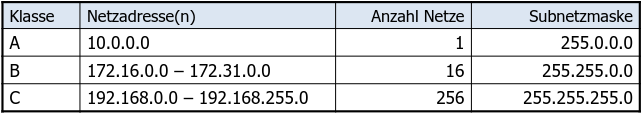
\includegraphics[width=0.9\linewidth, height=10mm]{private-ip}
\end{center}




